%%%%%%%%%%%%%%%%%%%%%%%%%%%%%%%%%%%%%%%%%%%%%%%%%%%%%%
% A Beamer template for Ritsumeikan University       %
% Author: Ming-Hao Xu (Xu Minghao)                   %
% Date:   April 2022.                                %
% LPPL Licensed.                                     %
%%%%%%%%%%%%%%%%%%%%%%%%%%%%%%%%%%%%%%%%%%%%%%%%%%%%%%

\documentclass{beamer}
\usepackage{hyperref}

\usepackage[UTF8]{ctex}
\usepackage[T1]{fontenc}

% other packages
\usepackage{latexsym,amsmath,xcolor,multicol,booktabs,calligra}
\usepackage{graphicx,pstricks,listings,stackengine}
\usefonttheme[onlymath]{serif}

% dummy text; remove it when working on this template
\usepackage{lipsum}

\author{Ebola}
\title{计算几何2:旋转卡壳、圆}
\institute{
    Institute of Mathematics, \\
    Zhejiang University.
}
\date{Jan, 2024}
\usepackage{Ritsumeikan}

% defs
\def\cmd#1{\texttt{\color{red}\footnotesize $\backslash$#1}}
\def\env#1{\texttt{\color{blue}\footnotesize #1}}
\definecolor{deepblue}{rgb}{0,0,0.5}
\definecolor{deepred}{rgb}{0.6,0,0}
\definecolor{deepgreen}{rgb}{0,0.5,0}
\definecolor{halfgray}{gray}{0.55}

\lstset{
    basicstyle=\ttfamily\tiny,
    keywordstyle=\bfseries\color{deepblue},
    emphstyle=\ttfamily\color{deepred},    % Custom highlighting style
    stringstyle=\color{deepgreen},
    numbers=left,
    numberstyle=\small\color{halfgray},
    rulesepcolor=\color{red!20!green!20!blue!20},
    frame=shadowbox,
}


\begin{document}

\begin{frame}
    \titlepage
\end{frame}

\begin{frame}
    \tableofcontents[sectionstyle=show,subsectionstyle=show/shaded/hide,subsubsectionstyle=show/shaded/hide]
\end{frame}

\section{基础回顾}

\begin{frame}[fragile]{向量的旋转}
    如果一个向量 $\overrightarrow{v}=(x,y)$,
    现在将它逆时针旋转 $90^\circ$,得到什么?

    \vspace{1em}\pause
    \begin{equation}
        \overrightarrow{v}^\perp=(-y,x).
    \end{equation}

\end{frame}

\begin{frame}[fragile]{点到直线的距离}
    \footnotesize
    给定 $P,A,B$ 三点坐标,求点 $P$ 到直线 $AB$ 的距离。(别用斜率)

    \vspace{1em}\pause
    \begin{figure}[H]
        \centering
        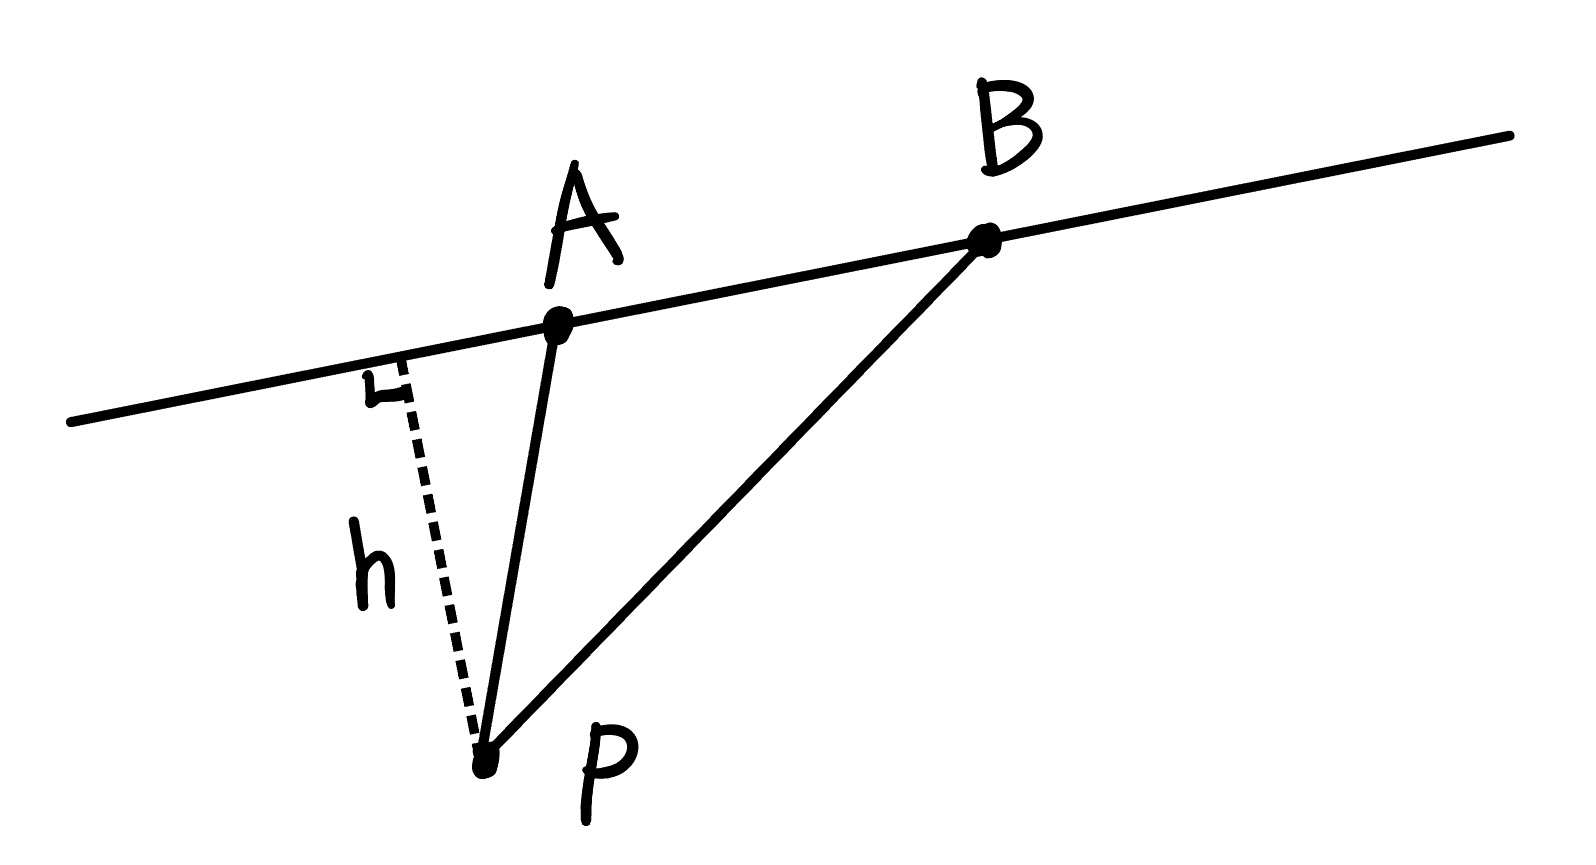
\includegraphics[width=0.5\textwidth]{pic/ptl.jpg}
    \end{figure}
    \begin{equation}
        h=\frac{S_{\Delta PAB}}{|AB|}=\frac{|\overrightarrow{PA}\times \overrightarrow{PB}|}{|AB|}.
    \end{equation}

    \vspace{1em}\pause
    \begin{lstlisting}[language=c++]
double DistanceToLine(Point P, Point A, Point B){
    return fabs(Cross(A-P, B-P)) / Length(A-B);
}
    \end{lstlisting}
\end{frame}

\section{旋转卡壳}

\begin{frame}{【模板】旋转卡壳}
    \small
    给定平面上 $n$ 个点,求凸包直径(直径是指最远的两个顶点的距离)。
\end{frame}

\begin{frame}{旋转卡壳}
    \small
    \begin{figure}[H]
        \centering
        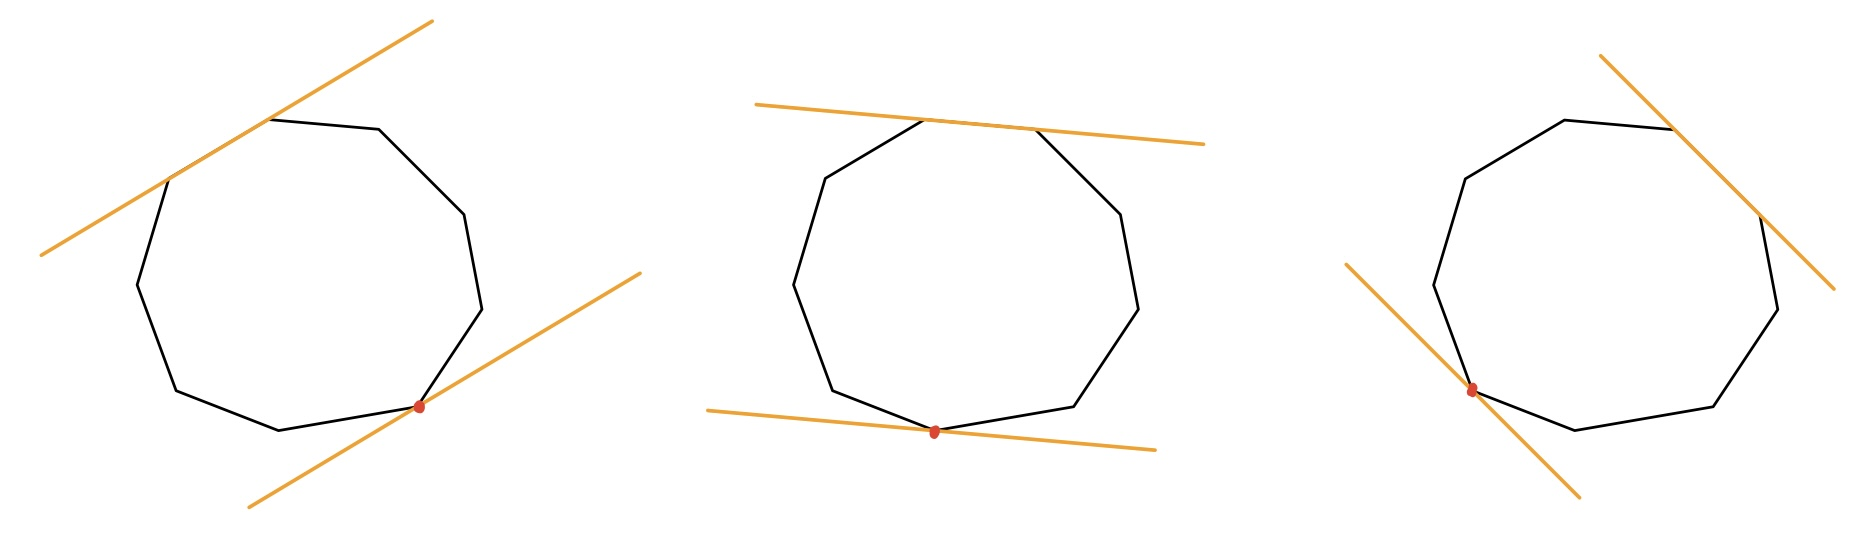
\includegraphics[width=\textwidth]{pic/rotation.jpg}
    \end{figure}
    如图所示,枚举上凸壳的边 $P_iP_{i+1}$,找到距离它最远的点。
    显然,当我们顺时针枚举边时,对面的点也只会顺时针方向前进,
    所以复杂度是 $O(n)$ 的。
\end{frame}

\begin{frame}[fragile]{旋转卡壳}
    \small
    \begin{lstlisting}[language=c++]
double RotatingCalipers(Point *ch, int n){
    if(n==2) return Length(ch[2] - ch[1]);
    int cur=0;
    double ans=0;
    ch[n+1] = ch[1];
    for(int i = 1; i <= n; i++){
        while(DistanceToLine(ch[cur], ch[i], ch[i+1]) 
           <= DistanceToLine(ch[cur%n+1], ch[i], ch[i+1])){
            cur = cur % n + 1;
        }
        ans=max(ans, max(Length(ch[i] - ch[cur]), 
                         Length(ch[i+1] - poly[cur])));
    }
    return ans;
}
    \end{lstlisting}
\end{frame}

\section{圆}

\begin{frame}{圆与直线的交点}
    \footnotesize
    给定直线上两个点 $A,B$ 的坐标、圆心 $P$ 的坐标、圆的半径 $r$,
    求直线 $l_{AB}$ 与圆的交点。

    \vspace{1em}\pause
    \begin{figure}[H]
        \centering
        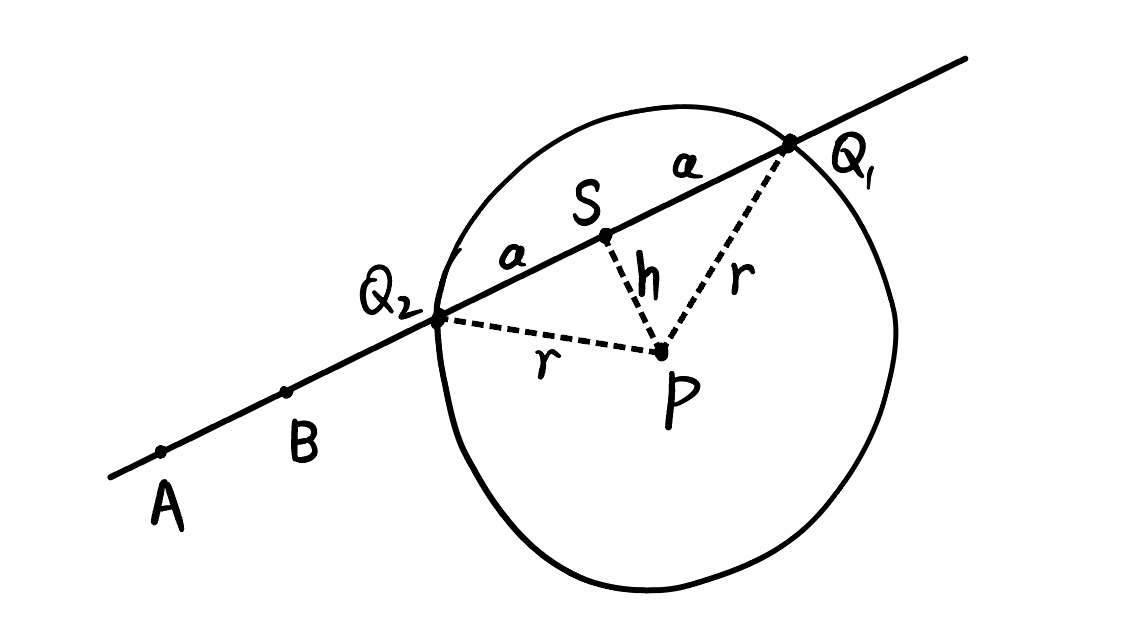
\includegraphics[width=0.4\textwidth]{pic/lineIcircle.jpg}
    \end{figure}
    先求出 $P$ 到 $l_{AB}$ 的距离 $h$,然后计算 $a=\sqrt{r^2-h^2}$,然后求出:
    \begin{align}
        S &= P+h \frac{\overrightarrow{AB}^\perp}{|AB|}\\
        Q_1 &= S + a \frac{\overrightarrow{AB}}{|AB|}\\
        Q_2 &= S - a \frac{\overrightarrow{AB}}{|AB|}\\
    \end{align}
\end{frame}

\begin{frame}{[BZOJ2178] 圆的面积并}
    给定 $n\;(n\leq 1000)$ 个圆,求它们覆盖区域的面积。
\end{frame}

\begin{frame}{[BZOJ2178] 圆的面积并}
    \footnotesize
    基本思路是辛普森积分求 $\int_L^R f(t)\; dt$,
    其中 $f(t)$ 表示直线 $x=t$ 与覆盖区域相交部分的长度。
    
    \vspace{1em}\pause
    对于一条直线 $x=t$,我们可以枚举所有圆,
    求出与该直线的所有交点,并从小到大排序,然后依次枚举;
    每碰到一个下交点,就加1,碰到上交点就减1;
    非零部分的总长度就是相交部分的长度。

    \begin{figure}[H]
        \centering
        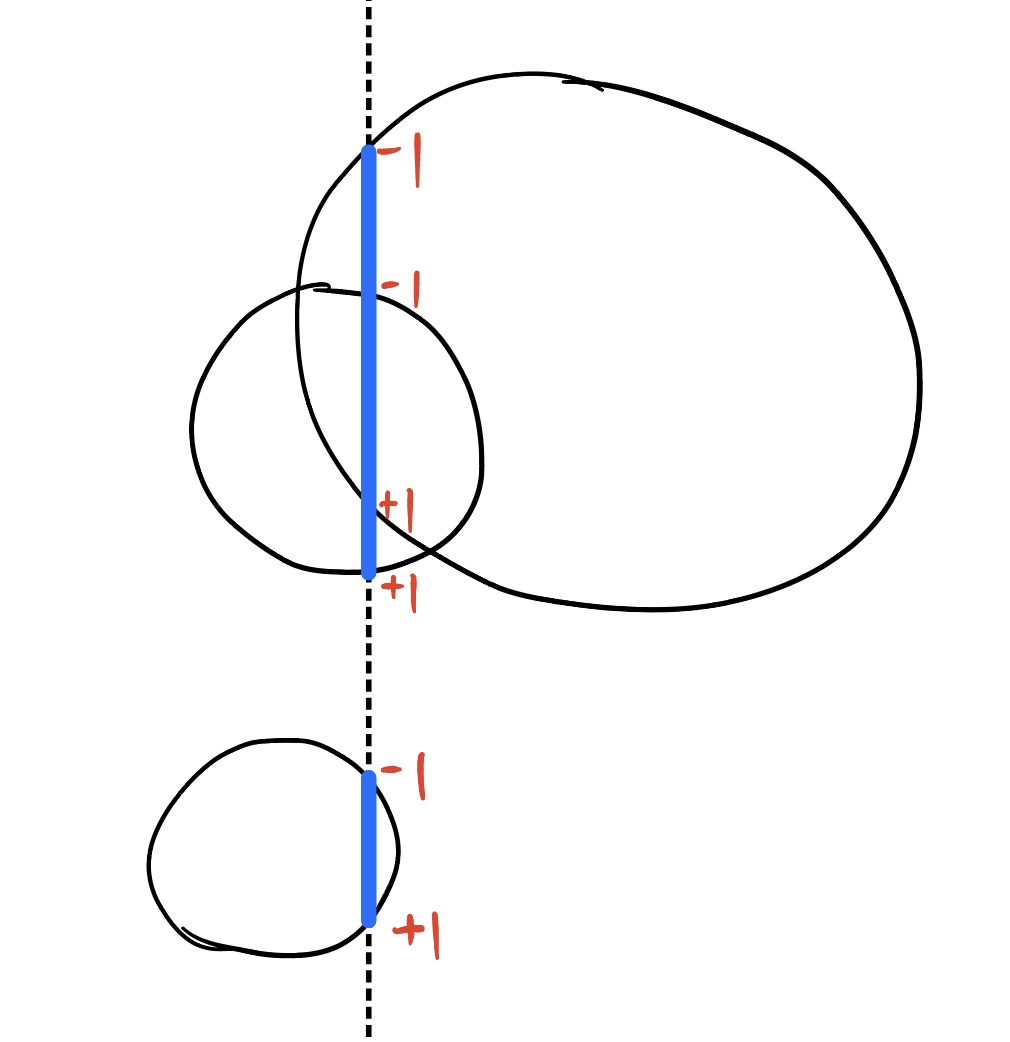
\includegraphics[width=0.4\textwidth]{pic/circleinsec.jpg}
    \end{figure}
\end{frame}

\begin{frame}{圆与圆的交点}
\end{frame}

\begin{frame}
    \begin{center}
        {\Huge\calligra Thank You}
    \end{center}
\end{frame}

\end{document}